\problemname{Triangeltal}
I en klass med $N$ elever har det blivit dags för det obligatoriska momentet att hålla tal. 
De flesta av eleverna ser fram emot att hålla tal väldigt mycket, och kan knappt vänta på sin tur.
Först måste de delas in i tre grupper. Alla i grupp $1$ kommer sedan presentera för grupp $2$, 
grupp $2$ för grupp $3$, och grupp $3$ för grupp $1$. 

Något som krånglar till den här gruppindelningen är att eleverna har olika ambitionsnivå. Varje elev $i$
kräver att få hålla tal inför minst $A_i$ personer.
Så om elev $i$ exempelvis hamnar i grupp $1$, så måste grupp $2$ ha minst $A_i$ medlemmar för att elev $i$ ska bli nöjd.

\begin{figure}[!h]
  \centering
  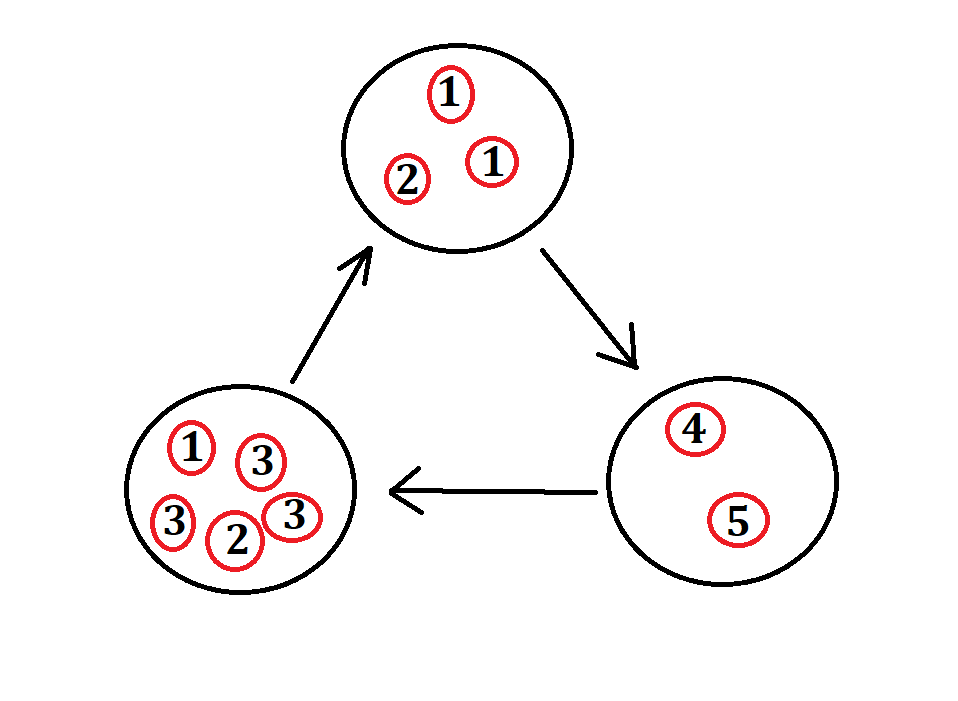
\includegraphics[width=6cm]{triangeltal.png}
  \caption{Bilden motsvarar första exemplet.}
\end{figure}

Din uppgift är att, givet elevernas ambitionsnivåer, avgöra om det finns ett sätt att dela in eleverna i tre grupper så att alla blir nöjda, och hitta i så fall en giltig indelning.

\section*{Indata}
Den första raden innehåller ett heltal $N$ ($3 \leq N \leq 5 \cdot 10^5$), antalet elever i klassen.

Den andra raden innehåller $N$ heltal $A_i$ ($1 \leq A_i \leq N$), där $A_i$ är antalet elever den $i$:te eleven minst vill hålla ett tal inför.

\section*{Utdata}
Om det inte finns en giltig indelning, skriv ut en enda rad med strängen ``\texttt{NO}''.

Om det finns en giltig indelning, skriv först ut en rad med strängen ``\texttt{YES}''. 
Skriv därefter ut en rad med en sträng $S$ bestående av tecknen \texttt{1}, \texttt{2} och \texttt{3}.
Tecknet på plats $i$ i denna sträng indikerar vilken grupp elev $i$ hamnade i. Om det finns flera lösningar
kan du skriva ut vilken som helst.

\section*{Poängsättning}
Din lösning kommer att testas på en mängd testfallsgrupper.
För att få poäng för en grupp så måste du klara alla testfall i gruppen.

\noindent
\begin{tabular}{| l | l | p{12cm} |}
  \hline
  Grupp & Poängvärde & Gränser \\ \hline
  $1$   & $14$       & $A_1 = A_2 = \cdots = A_N$\\ \hline
  $2$   & $16$       & $N \leq 10$  \\ \hline
  $3$   & $11$       & $A_i \leq 3$ \\ \hline
  $4$   & $23$       & $N \leq 3000$ \\ \hline
  $5$   & $36$       & Inga ytterligare begränsningar \\ \hline
\end{tabular}
